\chapter{Frozen Lake}
Frozen lake involves crossing a frozen lake from start to goal without falling into any holes by walking over the frozen lake. 
Frozen Lake is available into two versions: deterministic and non-deterministic setting the variable 
\begin{lstlisting}[language=Python, caption=slippery variable]
    is_slippery = True # Set the Non Deterministic environment
    is_slippery = False # Set the Deterministic environment
\end{lstlisting}
In the non-determinisitc environment the agent may not always move in the intended direction while in the determinisitc environment it always moves in the intended location.
In this project we use the simplest version of the Frozen Lake that is a {4x4} grid where the agent starts to position (0,0) with the goal located at the position (3,3).
Holes in the ice are distributed on the cells of the grid.
The agent makes moves until they reach the goal or fall in a hole.
The figure \ref{fig:frozen_lake_environment} shown an example ov the Frozen Lake environment:
\begin{figure}[h]
    \centering
    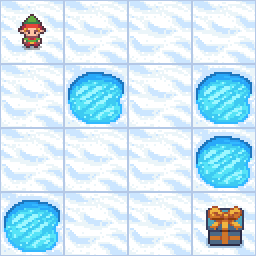
\includegraphics[width=0.5\textwidth]{images/image.png}
    \caption{Frozen Lake 4x4 environment}
    \label{fig:frozen_lake_environment}
\end{figure}
\newpage
\section{Action Space}
The agent has 4 possible actions to use:
\begin{itemize}
    \item 0: Move left
    \item 1: Move down
    \item 2: Move right
    \item 3: Move up
\end{itemize}
\section{Observation Space}
The observation is an integer value representing the current position of the agent.
The image in figure \ref{fig:frozen_lake_environment_observation_space} shown the observation space
\begin{figure}[h]
    \centering
    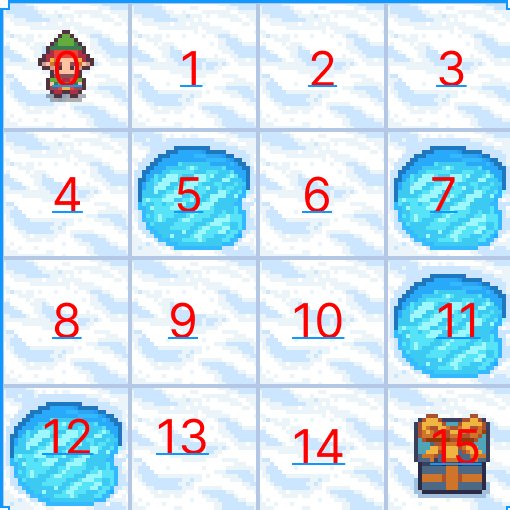
\includegraphics[width=0.5\textwidth]{images/observation_space.png}
    \caption{Frozen Lake 4x4 environment: Observation Space}
    \label{fig:frozen_lake_environment_observation_space}
\end{figure}
\section{Rewards}
The rewards are the feedback obtain by the agent while perform an action when it is a specific state.
The agent will try to maximize the rewards during the execution.
In this environment the rewards are:
\begin{itemize}
    \item Reach the goal $\rightarrow$ +1
     \item Reach the hole $\rightarrow$ 0
    \item Reach the frozen $\rightarrow$ 0
\end{itemize}
\section{Episode ends}
The episodes ends in the following cases:
\begin{itemize}
    \item Termination (The agent fall into hole or achieve the goal)
    \item Truncation (The time length of the episode, in this case is 100)
\end{itemize}
The condition of termination and truncation are given by the environment after agent takes an action

\section{Non-Deterministic environment}
We know in deterministic environement an action taken by the agent in a given state will go always in the expected destination state.
This is not true for the non-deterministic environment where if the agent wants to take the action "move left" it will taken with a 
\begin{equation}
    \Pr = \frac{1}{3} 
\end{equation}

\section{Brief of Q-Learning}
Reinforcement Learning (RL) is one of three basic machine learning ofmachine learning concerned with how an agent should take actions in a dynamic environment to maximize a reward. 
Finding a balance between exploration (of uncharted environment) and exploitation (of current knowledge) with the goal of maximize the cumulative reward. 
The environment is typically stated in the form of a Markov decision process (MDP).
The purpose of reinforcement learning is for the agent to learn an optimal policy that maximizes the reward function or other user-provided reinforcement signal that accumulates from immediate rewards.
\subsection{Agent's learning task}
A basic reinforcement learning agent interacts with its environment in discrete time steps. 
At each time step t, the agent receives the current state $S_t$ and reward $R_t$. 
It then chooses an action $A_t$ from the set of available actions, which is subsequently sent to the environment. 
The environment moves to a new state $S_{t+1}$ and the reward $R_{t+1}$ 
associated with the transition ($S_t$,$A_t$,$S_{t+1}$) is determined. 
The goal of a reinforcement learning agent is to learn a policy

\subsection{Q-Function}
The Q-Function (the state-action) function is a function that helps the agent to decide which action to take in a given state in order to maximize  its expected cumulative reward.
In general we can write the Q-Function using the Bellman equation:
\begin{equation}
Q(s, a) \leftarrow Q(s, a) + \alpha \left( r + \gamma \max_{a'} Q(s', a') - Q(s, a) \right)
\label{non_deteministic_q_function}
\end{equation}
\newline
\textbf{Q(s, a):} Current estimate of the expected cumulative reward for taking action \(a\) in state \(s\) and following the optimal policy thereafter.
\newline
\textbf{Q(s, a):} The current Q-value for the state-action pair \( (s, a) \).
\newline
\textbf{\(\alpha\):} The \textit{learning rate}. It controls how much the new information should override the old information. A higher value means the agent will quickly adapt to new experiences.
\newline
\textbf{r:} The \textit{immediate reward} received after taking action \(a\) in state \(s\).
\newline
\textbf{\(\gamma\):} The \textit{discount factor}. It determines how much the agent values future rewards compared to immediate rewards. A value close to 1 means the agent cares about long-term rewards, while a value close to 0 means the agent prioritizes immediate rewards.
\newline
\textbf{\(\max_{a'} Q(s', a')\):} The maximum Q-value over all possible actions \(a'\) in the next state \(s'\). This represents the best expected reward the agent can get from the next state onward.
\newline
\textbf{Q(s, a):} The original Q-value before the update, which is updated based on the new experience.

\subsection{Hyperparameters}
They are parameters set before the learning process begins, play a crucial role in determining the efficiency and effectiveness of the learning process. 
\begin{itemize}
    \item \textbf{Learning rate ($\alpha$)}: Controls how much the Q-values are adjusted during each update. A larger learning rate leads to faster updates, but can also result in instability. A smaller learning rate may lead to slower learning.
    \item \textbf{Discount factor ($\gamma$)}: Determines how much the agent values future rewards compared to immediate rewards. A discount factor close to 1 means the agent values long-term rewards, while a value close to 0 means the agent focuses on immediate rewards.
    \item \textbf{Exploration rate ($\epsilon$)}: In the $\epsilon$-greedy strategy, this parameter controls the probability with which the agent chooses a random action (exploration) instead of the action with the highest Q-value (exploitation). It helps balance exploration of new actions with exploiting the known best actions.
    \item \textbf{Number of episodes ($N$)}: Specifies the number of training episodes or iterations over which the agent will interact with the environment and learn. More episodes typically lead to better learning but require more computation time.
\end{itemize}
Choosing the right set of hyperparameters is crucial for training an effective model. Poor choices of hyperparameters can lead to slow convergence, overfitting, or even complete failure of the algorithm to learn useful behavior.

\section{Brief of DQN}

\section{Solving the Deterministic Environment}
\subsection{Deterministic Environment}
In a \textit{deterministic} environment, the outcome of any action taken by the agent is completely predictable.
For a given state \( s \) and action \( a \), the next state \( s' \) is always the same. 
The environment follows strict rules, meaning that there is no randomness involved in the transition from one state to another.
The reward associated with an action is also deterministic, meaning the agent always receives the same reward for performing the same action in the same state.
The agent can rely on complete predictability and plan its actions with full certainty about the consequences.
In deterministic environments, the Q-value can be updated directly based on the immediate reward and the known future reward, so \( \alpha \) isn't needed. 
Then the update rule for the Q-function is:
\begin{equation}
Q(s, a) \leftarrow r + \gamma  Q(s', a')
\label{deteministic_q_function}
\end{equation}

\subsection{Learning function}
The following algorithm shows the pseudocode of the learning function
\begin{algorithm}[H]
    \caption{Q-learning Algorithm (with $\varepsilon$-greedy)}
    \begin{algorithmic}[1]
    \State \textbf{Input:} discount factor $\gamma$, exploration rate $\varepsilon$, number of episodes $N$
    \State \textbf{Initialize:} Q-table $Q(s, a)$ for all states $s$ and actions $a$, set episode count $i = 1$
    \State \textbf{Initialize:} $\varepsilon_{min} \leftarrow 0.01$, $\varepsilon_{start} \leftarrow \varepsilon$, $k = 0.00001$
    
    \While{$i \leq N$}
        \State Initialize starting state $s_1$
        \While{not terminated or truncated $s_t$}
            \State Choose action $a_t$ based on the $\epsilon$-greedy policy:
            \If{random number $r \leq \epsilon$}
                \State Select a random action $a_t$ \Comment Exploration
            \Else
                \State Select action $a_t \leftarrow \arg\max_{a} Q(s_t, a)$ \Comment Exploitation
            \EndIf
            \State Take action $a_t$, observe reward $r_t$ and next state $s_{t+1}$
            \State $Q(s_t, a_t) \leftarrow r_t + \gamma Q(s_{t+1}, a')$ \Comment Update Q-Value
            \State $s_t \leftarrow s_{t+1}$
        \EndWhile
        \State $i \leftarrow i + 1$
        \State $\varepsilon \leftarrow \max\left(\varepsilon_{\text{min}}, \varepsilon_{\text{start}} \cdot e^{-k \cdot (i+1)}\right)$
    \EndWhile
    \State \textbf{Output:} $\pi \leftarrow \{s : \arg\max Q[s] \, | \, s \in \text{range}(\text{for all states s})\}$
\end{algorithmic}
\end{algorithm}
\subsubsection{Input parameters}
The algorithm takes in input the discount factor $(\gamma)$, the exploration rate $(\epsilon)$, the number of iterations (episodes) $N$.
\begin{itemize}
    \item \textbf{Discount factor ($\gamma$)} is a value  $ 0 \leq  \gamma \leq 1$. A discount factor close to 1 means the agent values long-term rewards, while a value close to 0 means the agent focuses on immediate rewards.
    \item \textbf{Exploration rate ($\epsilon$)} is a value  $ 0 \leq  \epsilon \leq 1 $ It helps balance exploration of new actions with exploiting the known best actions.
    \item \textbf{Number of episodes ($N$)} is an integer value  $ N \ge 1 $ It specifies the number of training with the agent that interacts with the environement
\end{itemize}
\subsubsection{Q-table}
In this environement instance the Q-table is represented as a matrix (2D array) composed by:
\begin{itemize}
    \item $4x4=16$ rows representing the \textbf{states}
    \item $4$ columns representing the \textbf{actions}
\end{itemize}
Then the final Q-Table is composed by $16x4=64$ elements
In this implementation the Q-Table is zeroized.
\subsection{Exploration and Exploitation strategy}
The agent will balance the exploration and the exploitation, we need to use a very high $\varepsilon$ parameter (closes to 1) to obtain an optimal policy.\\
During the iterations the algorithm will update $\varepsilon$ value using the formula:
\begin{equation}
    \label{exponential_decay}
    \varepsilon \leftarrow \max\left(\varepsilon_{\text{min}}, \varepsilon_{\text{start}} \cdot e^{-k \cdot (i+1)}\right)
\end{equation}
\subsection{Output}
In output the agent will return the policy learned, and the Q-Table updated.
\subsection{Results}
We learned three agents with different parameters, and collected cumulative rewards during the learning phase then the following are the results:
\begin{figure}[h]
    \centering
    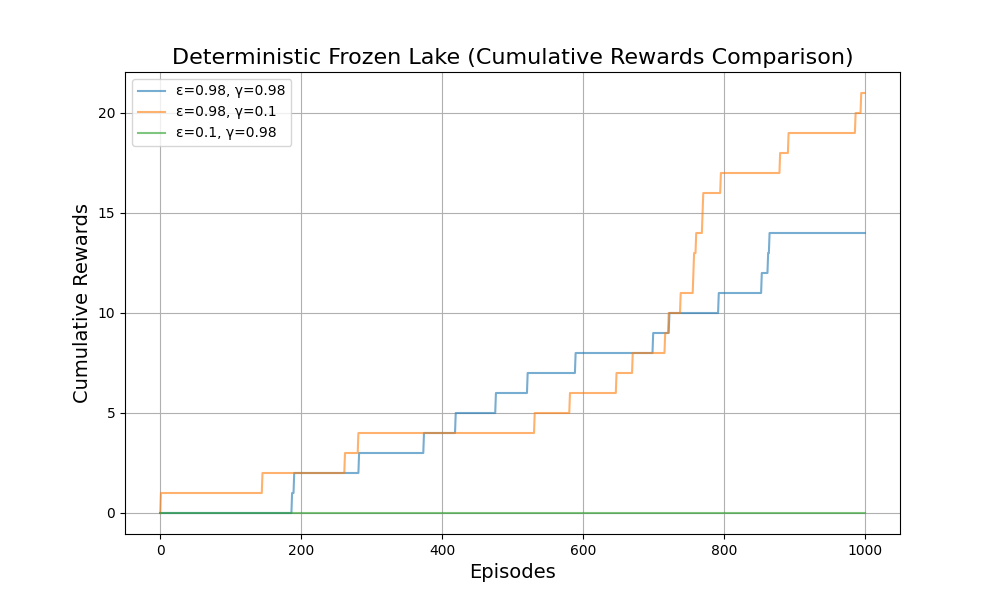
\includegraphics[width=0.99\textwidth]{images/cumulative_rewards_deterministic_comparison.png}
    \caption{Agents comparison}
    \label{fig:cumulative_rewards_deterministic_comparison}
\end{figure}
From the \ref{fig:cumulative_rewards_deterministic_comparison} we can see:
\begin{itemize}
    \item The green agent (with $\varepsilon = 0.1$) will not reach out the optimal policy, because the agent prefers exploitation instead of balance with exploration
    \item The orange agent has an high $\varepsilon = 0.98$ that allows the agent to balance exploitation and exploration. The second parameter $\gamma=0.1$ indicates, that the agent prefers immadiate reward to future reward, and we can see the learning process start immediatly.
    \item The blu agent has $\varepsilon = 0.98$ that allows to balance exploitation and exploration. The second parameter $\gamma=0.98$ indicates, that the agent prefers future rewards to immediate rewards, and we can see the learning process starts after some episodes.
\end{itemize}
We can see an highlight of the Q-Table learned by agents (blue and green agents) that help us to understand the final Q-Table learned by the two agents
\begin{figure}[H]
    \centering
    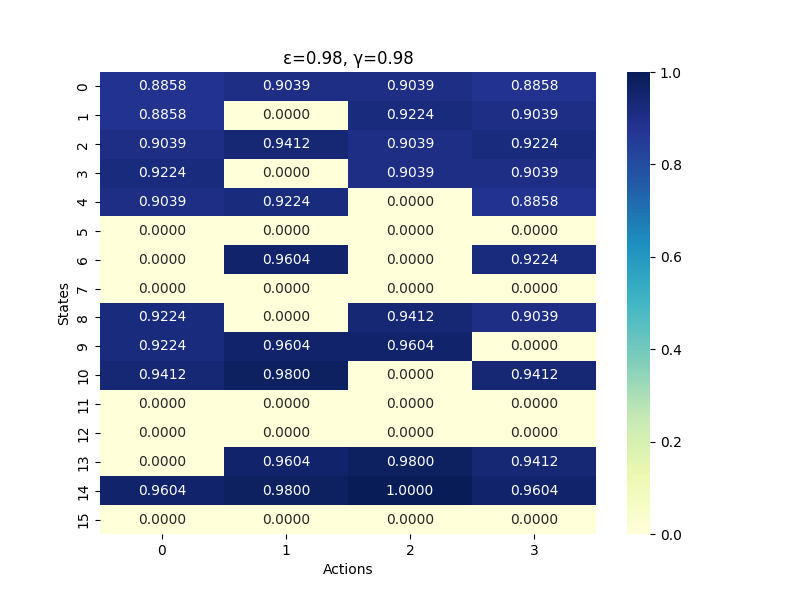
\includegraphics[width=0.99\textwidth]{images/heatmap1.png}
    \caption{Q-Table of blue agent}
    \label{fig:blue_agent}
\end{figure}
\begin{figure}[H]
    \centering
    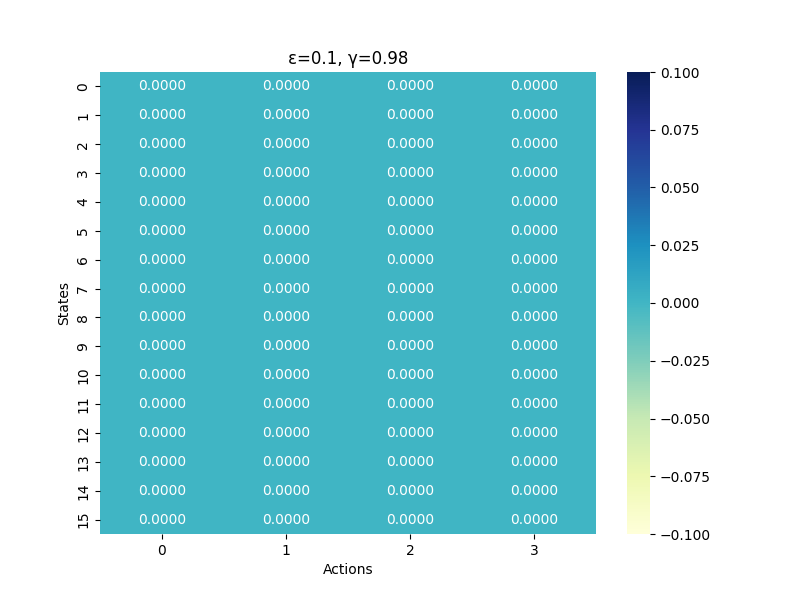
\includegraphics[width=0.99\textwidth]{images/heatmap3.png}
    \caption{Q-Table of green agent}
    \label{fig:green_agent}
\end{figure}
Using the policies learned by the agents is possible to see success rate that in a deterministic environement must be 100\%
In the figure \ref{fig:success_rate_log} are shown the $\log(\frac{wins}/{episodes})$ of the three agents:
\begin{figure}[H]
    \centering
    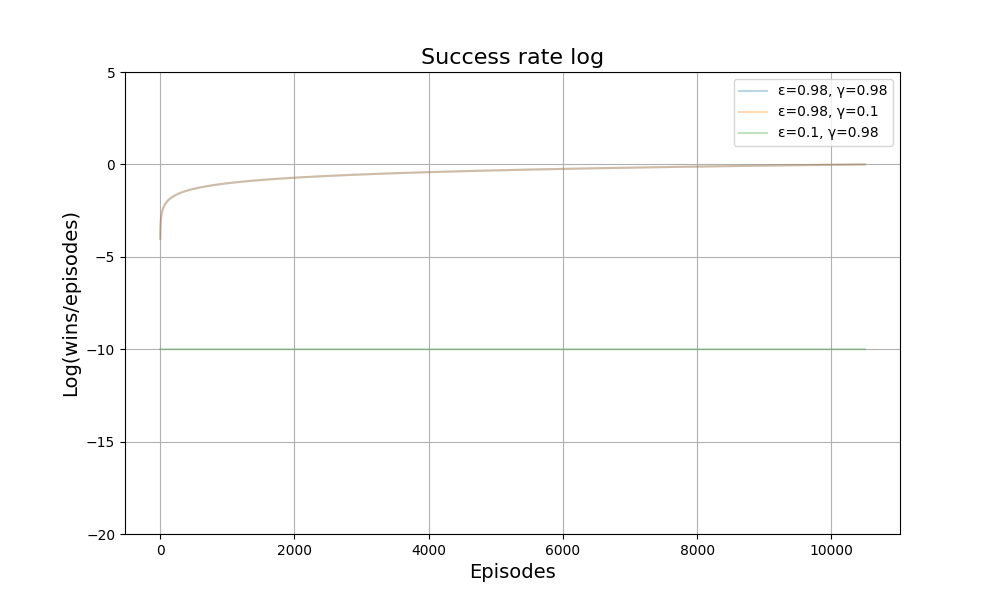
\includegraphics[width=0.99\textwidth]{images/success_rate_log.png}
    \caption{Success rate log}
    \label{fig:success_rate_log}
\end{figure}

\begin{itemize}
    \item The green agent has no rewards and for convenience is designed as a constant negative line, because it never converges to the optimal policy
    \item The other two learned agents are overlapping (you can see the brown curve that is the union of the blue and orange), and they converge to the optimal policy
\end{itemize}
\section{Solving the Non-Deterministic Environment}
\subsection{Learning Function}
The following algorithm shows how the agent is learned in a non-deterministic environment
\begin{algorithm}[H]
    \caption{Q-learning Algorithm (with $\varepsilon$-greedy)}
    \begin{algorithmic}[1]
    \State \textbf{Input:} discount factor $\gamma$, exploration rate $\varepsilon$, learning rate $\alpha$, number of episodes $N$
    \State \textbf{Initialize:} Q-table $Q(s, a)$ for all states $s$ and actions $a$, set episode count $i = 1$
    \State \textbf{Initialize:} $\varepsilon_{min} \leftarrow 0.01$, $\varepsilon_{start} \leftarrow \varepsilon$, $k = 0.00005$
    \While{$i \leq N$}
        \State Initialize starting state $s_1$
        \While{not terminated or truncated $s_t$}
            \State Choose action $a_t$ based on the $\epsilon$-greedy policy:
            \If{random number $r \leq \epsilon$}
                \State Select a random action $a_t$ \Comment Exploration
            \Else
                \State Select action $a_t \leftarrow \arg\max_{a} Q(s_t, a)$ \Comment Exploitation
            \EndIf
            \State Take action $a_t$, observe reward $r_t$ and next state $s_{t+1}$
            \State $Q(s, a) \leftarrow Q(s, a) + \alpha \left( r + \gamma \max_{a'} Q(s', a') - Q(s, a) \right)$ \Comment Update Q-Value
            \State $s_t \leftarrow s_{t+1}$
        \EndWhile
        \State $i \leftarrow i + 1$
        \State $\varepsilon \leftarrow \max\left(\varepsilon_{\text{min}}, \varepsilon_{\text{start}} \cdot e^{-k \cdot (i+1)}\right)$
    \EndWhile
    \State \textbf{Output:} $\pi \leftarrow \{s : \arg\max Q[s] \, | \, s \in \text{range}(\text{for all states s})\}$
\end{algorithmic}
\end{algorithm}
\subsubsection{Difference}
In non-determinisitic environment we have another input parameter the learning rate.
It controls how much the Q-values are adjusted during each up-date. A larger learning rate leads to faster updates, but can also result in instability.
\begin{itemize}
    \item $\alpha$ closes to 0 the learning rate is very slow, but the Q-Table will have stable values.
    \item $\alpha$ closes to 1 the learning rate is fast, but the Q-Table will have unstable values.
\end{itemize}
Another important difference is the Q-Function used, that in this case is \ref{non_deteministic_q_function}
\subsection{Results}
Now we can see the results of three learned agents.
\begin{figure}[H]
    \centering
    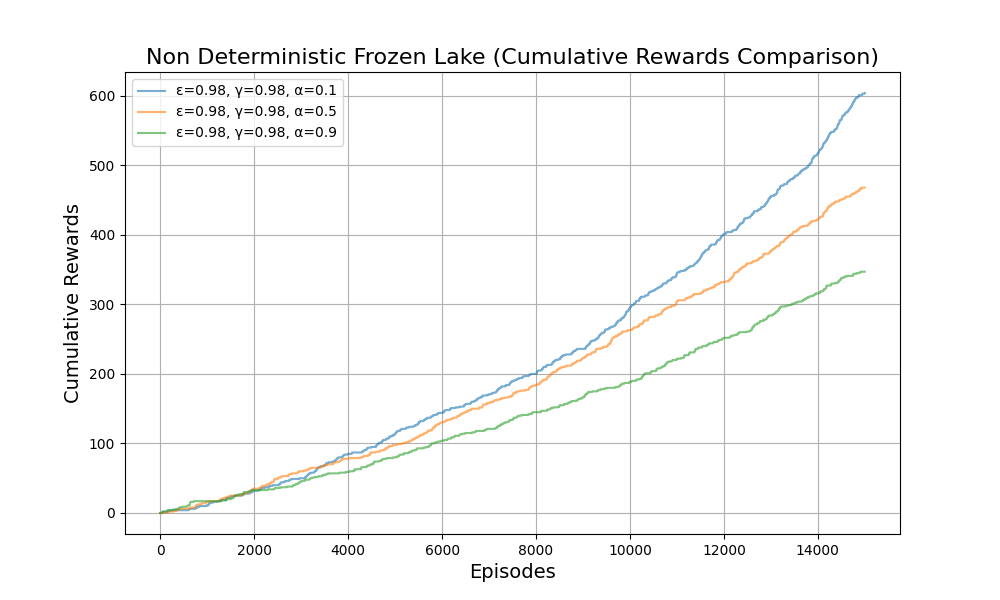
\includegraphics[width=0.99\textwidth]{images/cumulative_rewards_non_deterministic_comparison.png}
    \caption{Agents comparison}
    \label{fig:cumulative_rewards_non_deterministic_comparison}
\end{figure}
In this analysis we are interesting to understand the learning rate parameter and how it changes the learning curve of the agents.
\begin{itemize}
    \item The blu agent has $\alpha=0.1$, this means that the agent will update with caution the new Q-Values, this causes a slow initial grows, but after a specific point, it will converge most speedly then each other to the convergence.
    \item The orange agent has $\alpha=0.5$, and it represent the balanced situation between the two curves, it will increase most speedly at begin of the blue agent, but it will converge slowly the the blue agent, but speedly then the green agent
    \item The green agent has $\alpha=0.9$, it will learn speedly to the begin, but this lead instability then it will reach the optimal policy most slowley then the other curves.
\end{itemize}
In the following picture are shown the Q-Table learned by the three agents:
\begin{figure}[H]
    \centering
    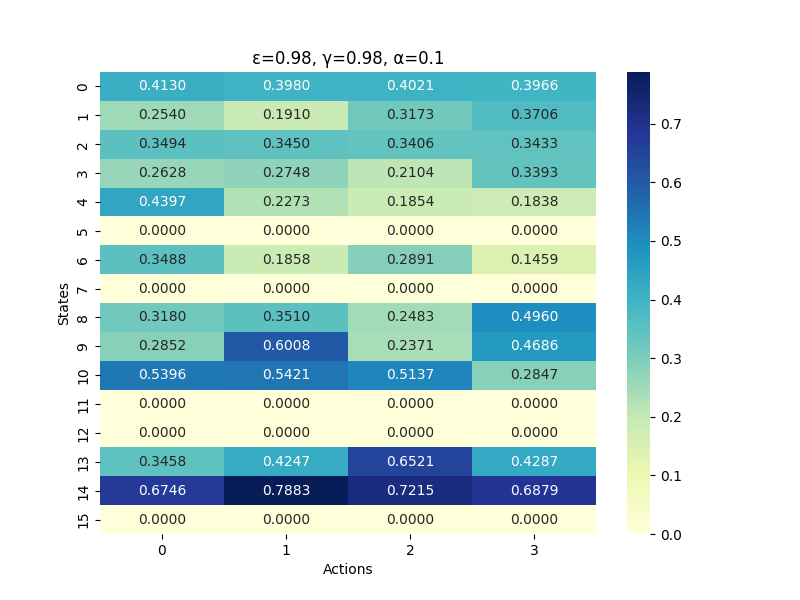
\includegraphics[width=0.99\textwidth]{images/heatmap_nd1.png}
    \caption{Q-Table of blue agent}
    \label{fig:blue_agent_nd}
\end{figure}
\begin{figure}[H]
    \centering
    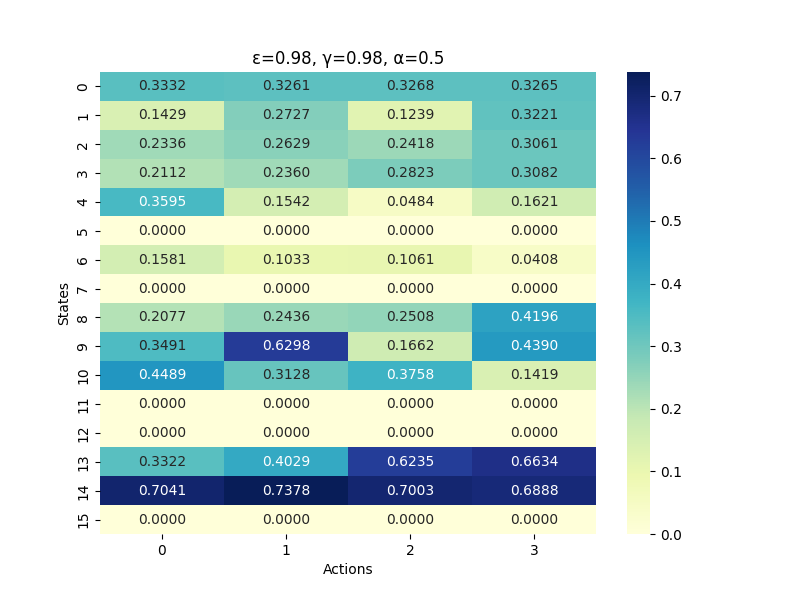
\includegraphics[width=0.99\textwidth]{images/heatmap_nd2.png}
    \caption{Q-Table of orange agent}
    \label{fig:orange_agent_nd}
\end{figure}
\begin{figure}[H]
    \centering
    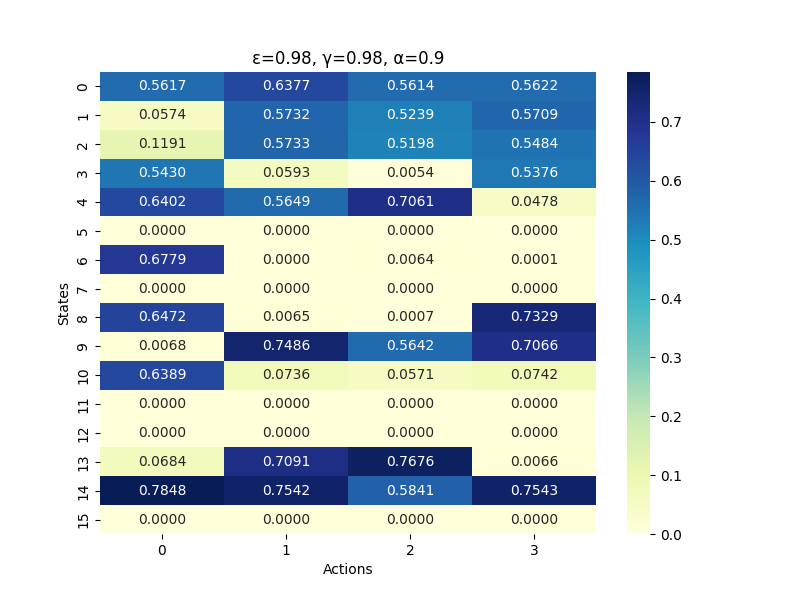
\includegraphics[width=0.99\textwidth]{images/heatmap_nd3.png}
    \caption{Q-Table of green agent}
    \label{fig:green_agent_nd}
\end{figure}
The obtained result end with the measure of the success rate.
In the following figure is shown the overlap success rate of three agents.
A very important fact is the agents learned an optimal policy, they do not have a success rate of 100\%.
\begin{figure}[H]
    \centering
    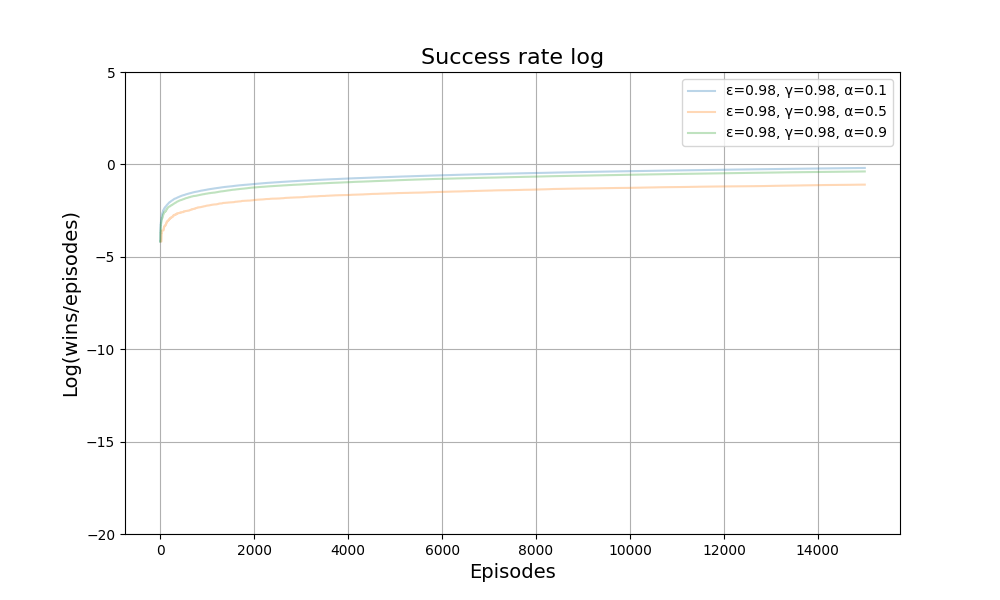
\includegraphics[width=0.99\textwidth]{images/success_rate_log_nd.png}
    \caption{Success rate log}
    \label{fig:success_rate_log_nd}
\end{figure}
